\chapter{Introduction}
\label{chp:introduction}

Development of complex systems requires an efficient way for engineers to ensure the correctness of the developed software. Domain Specific Modeling (DSM) can achieve this through automatic code generation and block-diagram visualizations, thus significantly reducing the risk of faulty applications and enabeling engineers to work more effectively.\\
In safety-critical development processes however, DSM can only be used without subsequent manual verification, if the DSM tools work correctly. This can either be achieved through time intensive qualified software development processes, which ensure accurate and reliable visualization of DSM through the tool itself, or through the use of unverified DSM tools followed by the subsequent use of a small visualization verification tool to ensure the correctness of the application.\\
In low-cost projects with high safety requirements, a cost-effective qualification method is crucial, highlighting the potential of the latter approach for a qualifiable graphical verification tool for use in DSM.

The Institute for Aircraft Systems is currently developing a way for avionic models to be developed inside a web-based graphical model editor called \textit{eXtensible Graphical EMOF Editor} or \textit{XGEE}.\\
XGEE uses three kinds of \textit{tokens} within three distinct editors to visualize avionic models. They are:
\begin{itemize}
    \item signals
    \item vertices
    \item text labels
\end{itemize}

\begin{figure}[h]
    \centering
    % First image
    \begin{subfigure}{0.3\textwidth}
        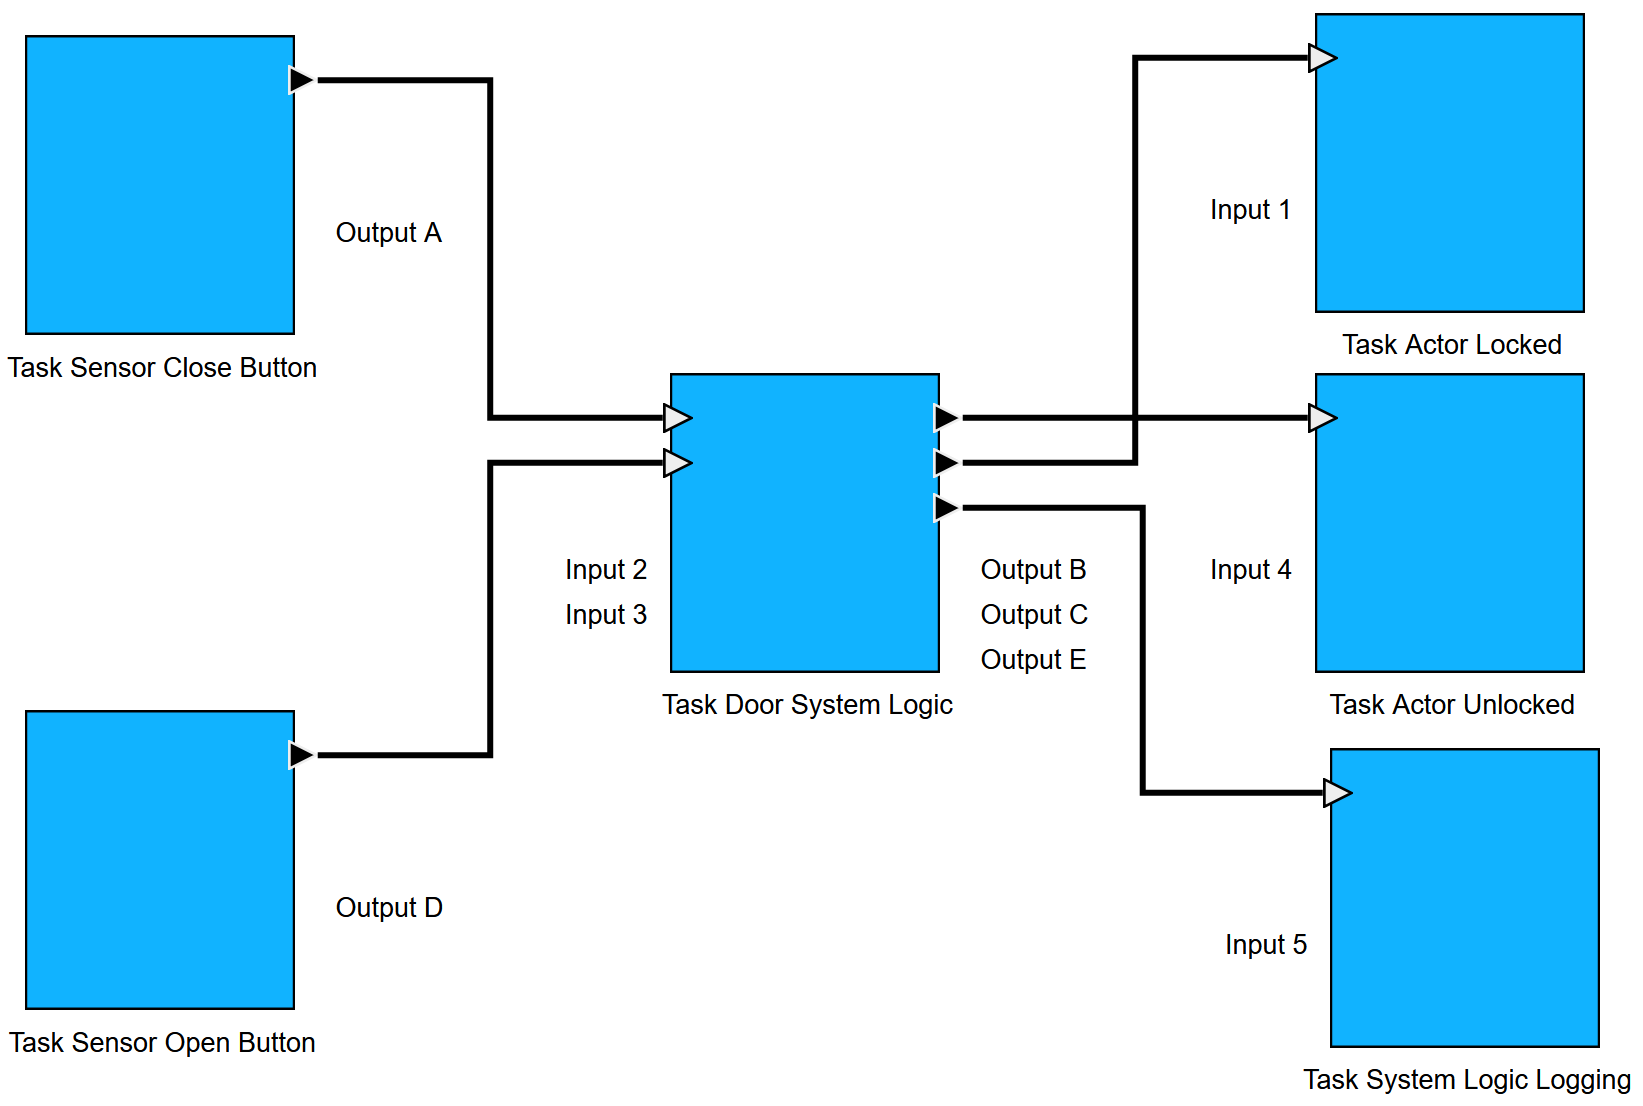
\includegraphics[width=\linewidth]{Pictures/functions_editor.png}
        \caption{Functions editor}
        \label{fig_functions_editor_en}
    \end{subfigure}
    \hfill
    % Second image
    \begin{subfigure}{0.3\textwidth}
        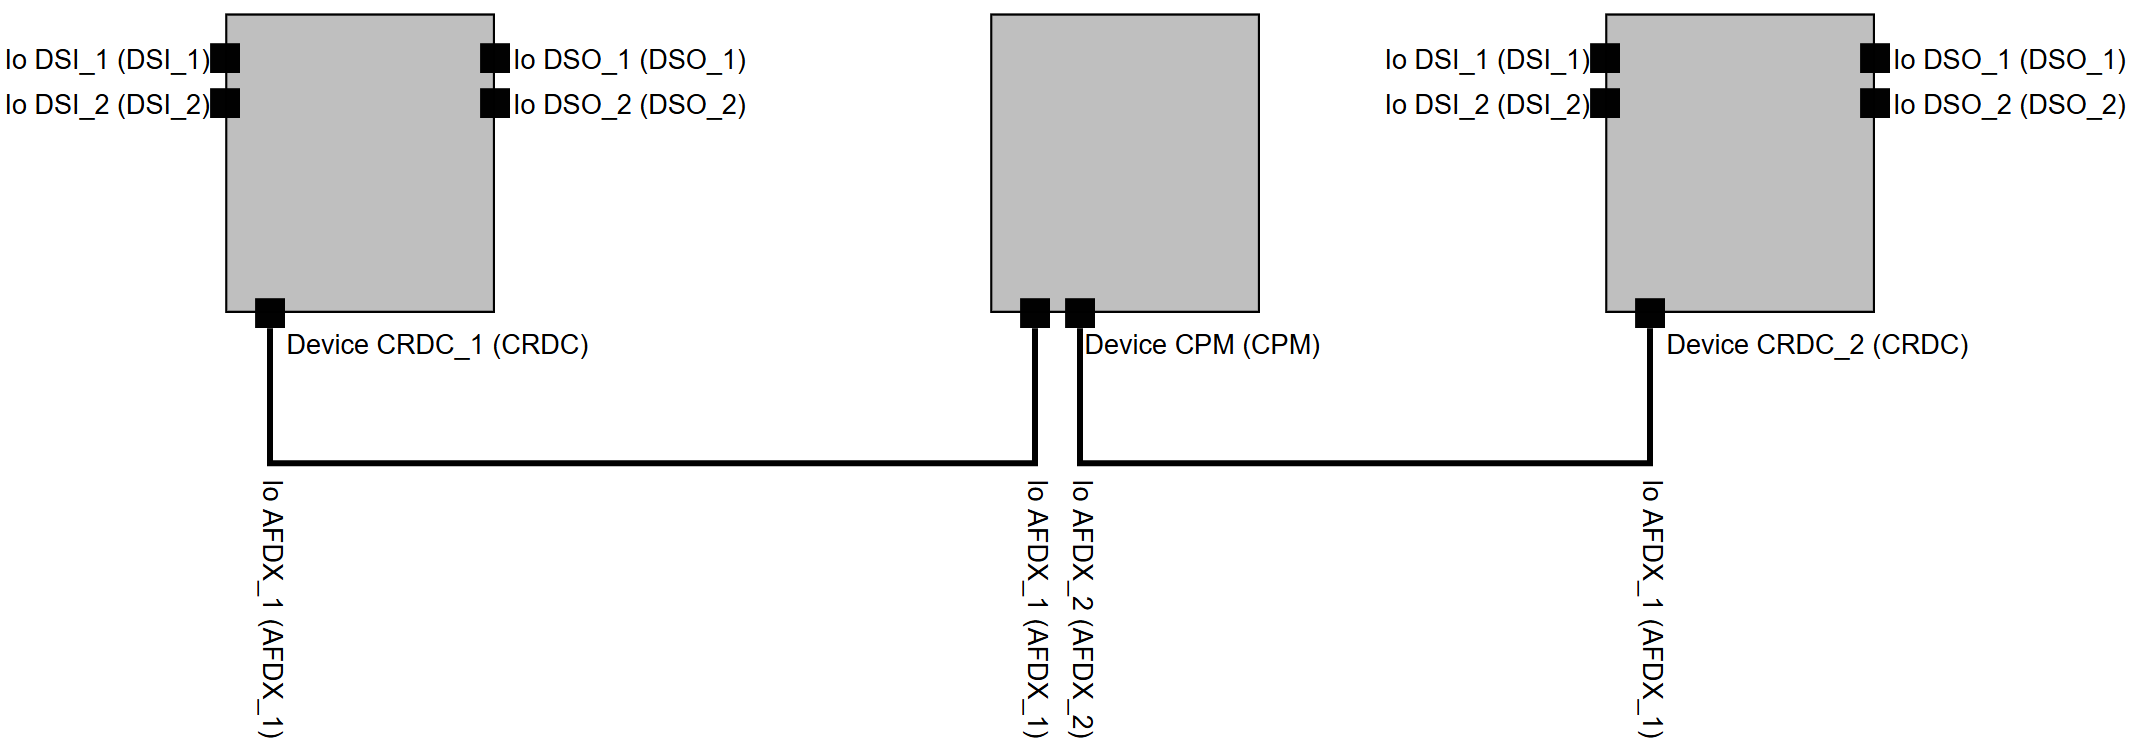
\includegraphics[width=\linewidth]{Pictures/hardware_editor.png}
        \caption{Hardware editor}
        \label{fig_hardware_editor_en}
    \end{subfigure}
    \hfill
    % Third image
    \begin{subfigure}{0.3\textwidth}
        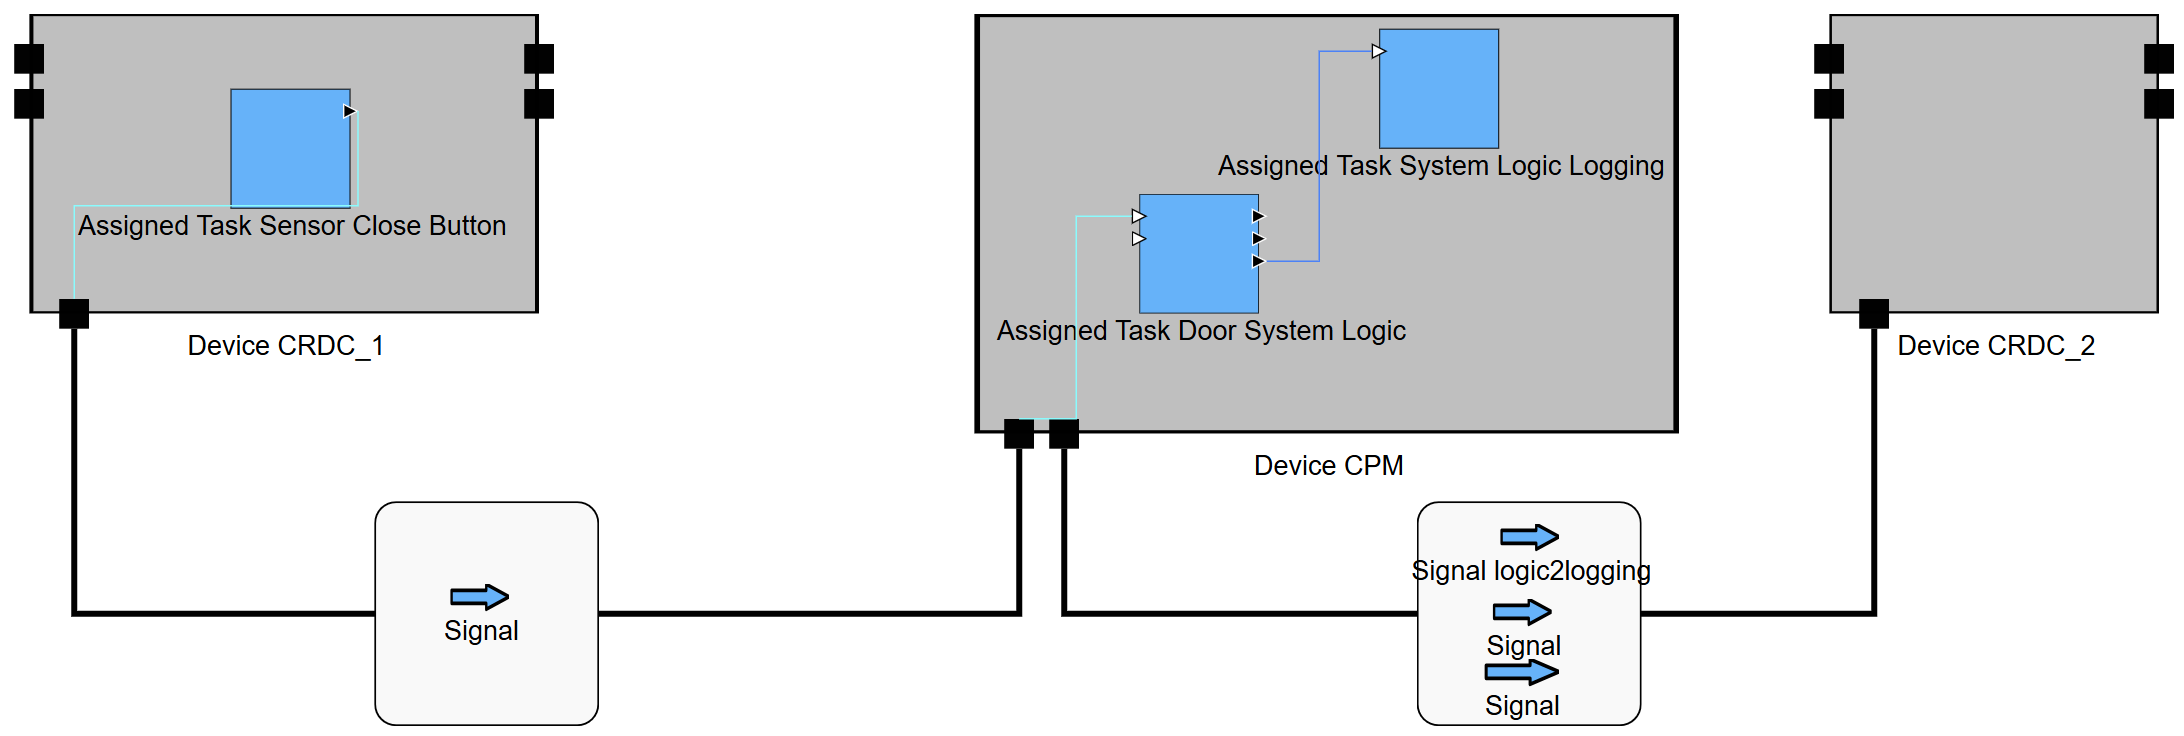
\includegraphics[width=\linewidth]{Pictures/allocations_editor.png}
        \caption{Allocations editor}
        \label{fig_allocations_editor_en}
    \end{subfigure}

    \caption{Functions- Hardware- and Allocations editors}
    \label{fig_editors_en}
\end{figure}
This paper builds upon the work of \cite{og_paper} to automate the verification process within XGEE by tokenizing a screenshot from within the editor. This means detecting the bounding boxes and token types of all elements of the diagram. To recognize and process the screenshot data, methods from the \textit{OpenCV } Python library are being used.\\
By rebuilding a model from the recognized tokens and comparing it to the original, visualization errors become apparent and can be indicated to the user, including issues such as unclear signal intersections, signals being obscured by blocks, text labels being obscured by signals or blocks, blocks being scaled down to the point of disappearing, or blocks obscuring other blocks.\\
The goal of this thesis is to provide a tool that can be used to verify the correctness of the visualization of avionic models within XGEE, thus enabling engineers to work more effectively and with a higher degree of confidence.


\section{Overview of Computer Vision}
What to Write: Define computer vision and its role in modern applications.
Mention its significance in interpreting visual data and extracting structured information.
Briefly touch on key algorithms and tools (e.g., OpenCV, deep learning in vision).



\section{Domain Specific Modeling (DSM)}
What to Write: Explain DSM and its purpose in creating specialized models for particular domains.
Describe how XGEE leverages DSM to simplify and automate diagram-based design processes.
Provide examples of DSM in real-world applications.
\section{The Role of Visualization in Diagram-Based Systems}
What to Write: Discuss why accurate diagram visualization is essential for tools like XGEE.
Highlight the challenges of interpreting complex diagrams with overlapping elements and multiple scales.
\section{Challenges in XGEE's visualization verification}
What to Write: Summarize the primary issues in the XGEE editor that motivated your work, such as edge detection, vertex identification, and text recognition.
Set the stage for the methods you implemented to overcome these challenges.
\section{State of the Art}



This chapter reviews the existing research and tools related to diagram interpretation, edge detection, vertex detection, and text recognition. By highlighting their strengths and limitations, this chapter establishes the need for the methods developed in XGEE.